\documentclass{article}
\usepackage[dutch]{babel}
\usepackage[utf8]{inputenc}
\setlength{\parskip}{\baselineskip}%
\setlength{\parindent}{0pt}%
\usepackage{listings}
\usepackage{graphicx}
\usepackage{amsmath}
\usepackage{hyperref}
\graphicspath{ {./images/} }

\usepackage[toc,page]{appendix}

\usepackage{minted}

\title{%
    Project Logisch Programmeren\\
    \large Implementeren van het spel Con-Tac-Tix
    }
\author{ Victor Matthijs }
\date{Juni 2020}

\begin{document}
\pagenumbering{gobble}
\maketitle
\newpage

\pagenumbering{Roman}
\tableofcontents
\newpage

\pagenumbering{arabic}
\section{Introductie}

Dit jaar is het project voor Logisch programmeren het implementeren van het project Con-Tac-Tix. Dit spel wordt gespeeld op een ruitvormig bord, waar elke tegel wordt voorgesteld door een hexagonaal. De borden waarmee we spelen kunnen verschillen van dimensies, maar het meest voorkomende bord is 11 x 11. De zijdes van het bord worden verdeeld tussen 2 spelers, deze 2 spelers kunnen elk een kleur kiezen en krijgen dan ofwel boven- en onderzijde of rechter- en linkerzijde. Elke speler mag om de beurt één tegel op het board plaatsen, dit mag om het even waar zijn op het board, maar niet op plaatsen waar er al een kleur ligt. Het spreekt voor zich dat een speler enkel zijn eigen kleur mag leggen op het bord. \newline
Het doel van het spel is om als eerste een pad te vormen die van de ene zijde naar de andere zijde van het bord loopt. Men moet dus de 2 zijdes met hun kleur verbinden. Men moet er hier dus voor zorgen dat elke tegel op hun pad een andere tegel aan een van de zijdes van de hexagoon raakt, anders heeft men geen pad en kan men dus ook niet winnen. \newline
\break
Het spel wordt geïmplementeerd als een input-output programma, we aanvaarden dus een invoerFile met een bepaalde structuur. Deze file zal geparsed worden naar een interne bord voorstelling, waarna het algoritme de beste zet zal terug geven. \newline
\break
Men kan het programma oproepen aan de hand van het volgende commando: 
\begin{lstlisting}[language=bash]
  $ cat invoerFile | swipl -f none -t halt -g main -q main.pl
  \end{lstlisting}
Het programma aanvaardt verschillende argumenten, deze worden hieronder toegelicht:
\begin{itemize}
  \item (No Arguments) : Wanneer het commando wordt uitgevoerd zonder argumenten mee te geven, dan zal het algoritme de beste zet teruggeven. Wanneer men in één stap kan winnen, dan zal het programma ook de winnende zet teruggeven.
  \item TEST: Het test argument zorgt ervoor dat het programma alle mogelijke zetten zal teruggeven vanuit de beginpositie van het bord. Al deze borden worden naar de standaar output geschreven.
  \item SVG: Het svg argument zorgt ervoor dat de oplossing van het algoritme terug wordt gegeven via SVG's, dit kunnen één of meerdere borden zijn.
\end{itemize}

Bovenstaande argumenten kunnen met elkaar worden gebruikt. 

\section{Hoe zit het spel in elkaar?}

Het spel begint zoals eerder is aangegeven, wanneer er een juist commando wordt ingegeven in de terminal. De eerste stap die moet gebeuren is het parsen van de $invoerFile$, deze file heeft een bepaalde structuur zoals weergegeven in de opgave op Ufora. De parser zelf zal gebruik maken van Prolog DCG (Prolog Definite Clause Grammer). \newline
De manier waarop het spel intern voorgesteld wordt is als het volgt: De parser zal de invoerFile overlopen en zal alle verschillende velden afhandelen. Er wordt binnen het programma met twee voorstellingen gewerkt, één daarvan zal het spel zelf voorstellen, dit ziet eruit als volgt: 
$$
game(Size, Turn, State, Ori, Tiles)
$$
De file die instaat voor het parsen van de input zal deze Game voorstelling ook terug geven aan de Main regel. Deze Game voorstelling zal dan daarna gebruikt worden om het effectieve bord voor te stellen. Ik heb ervoor gekozen om het bord als een matrix voor te stellen (List of Lists). Hier zullen de lege plaatsen van het bord worden voorgesteld door een 0, en de andere plaatsen worden ingenomen door de naam van de kleur. 
Aan de hand van deze 2 voorstelling is de rest van het programma ook opgebouwd, alles start vanuit de main module. Hier wordt er gekeken naar welke argumenten meegegeven werden met het commando.\newline
Een voorbeeld van deze voorstelling kan men hieronder zien:\newline
\begin{center}
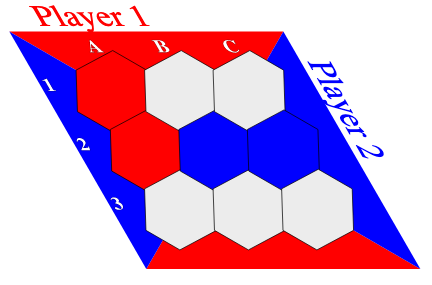
\includegraphics[scale=0.4]{board}
\end{center}
\[
M=
  \begin{bmatrix}
    red & 0 & 0 \\
    red & blue & blue \\
    0 & 0 & 0
  \end{bmatrix}
\]

De rest van het programma wordt verder opgedeeld in verschillende modules, naast de main module is er ook nog een game, board, minimax\_ai, parser en SVG module. Deze opsplitsing zorgt ervoor dat het programma duidelijk en gestructureerd blijft. Al deze modules worden ook ondersteund doormiddel van commentaar bij elke (logische) regel. Wat volgt zijn hele kleine beschrijvingen van wat elke module precies doet.

\subsection{Parser Module}
Dit is de eerste module die wordt opgeroepen vanuit de main. Deze module zal ook maar één regel/predicaat exporteren via het PublicList argument. Alles start vanuit de parse regel op lijn 45. Deze regel zal deel van de invoerFile als een apart $game\_part$ behandelen. Ik heb de code zo geschreven dat de verschillende $game\_parts$ in verschillende volgordes kunnen voorkomen. Hier wordt ook telkens rekening gehouden met de mogelijke whitespaces en newlines die kunnen voorkomen in de invoerFile.
\inputminted[firstline=42, lastline=56, linenos, breaklines]{prolog}{/Users/Victor/Documents/UGent/3BI/Logisch/Project/project/src/parser.pl}
Zoals eerder aangegeven maakt deze parser module gebruik van Prolog Definite Clause Grammer. Ik heb hier ook zoveel mogelijk gebruik proberen maken van de basic DCG regels die beschikbaar zijn door Prolog. De bedoeling van deze parser module is dus om de invoerFile om te zetten naar een Game representatie zoals eerder aangehaald is. Deze representatie zal dan gebruikt worden bij het verdere verloop van het spel.

\subsection{Game Module}
De Game module is één van de twee modules die de representatie van het spel afhandelen, zoals de naam al prijs geeft zal deze module dus alle regels en predicaten bevatten voor een game. Wat volgt zijn een paar belangrijke aspecten die in deze module aanwezig zijn.
\begin{itemize}
  \item Het eerste belangrijke wat deze module bevat zijn regels die ervoor zorgen dat de argumenten van onze game toegankelijk zijn tijdens het minimax algoritme. Deze verschillende regels bevinden zich op lijn 16-72.
  \item Lijn 73-125 bevat de logica voor het afprinten van de games naar de gebruiker. Al deze regels zullen worden opgeroepen wanneer er geen SVG argument is meegegeven. Hier zal dus de regel $print\_all\_games$ elke game representatie die het krijgt afprinten naar standaard output/terminal.
\inputminted[firstline=94, lastline=102, linenos, breaklines]{prolog}{/Users/Victor/Documents/UGent/3BI/Logisch/Project/project/src/game.pl}
\item Het laatste deel van deze module bevat regels voor het maken van nieuwe game representatie uitgaande van een bord of oude game. De regel $create\_game\_from\_board$ wordt opgeroepen vanuit de main nadat het minimax algoritme klaar is. Deze regels zijn te vinden op lijn 126-200.
\inputminted[firstline=147, lastline=152, linenos, breaklines]{prolog}{/Users/Victor/Documents/UGent/3BI/Logisch/Project/project/src/game.pl}

\end{itemize}

\subsection{Board Module}
Een andere module die wordt opgeroepen vanuit de main is de Board module. Deze module beschikt over alle regels die te maken hebben met het Con-Tac-Tix spelbord en de spelregels er rond. Na het parsen van de invoerFile zal de $construct\_board\_from\_tiles$ worden opgeroepen vanuit de main. Deze zal een list van tiles meegeven als argument, en het zal een matrix vormen met alle tiles op de juiste plaats. Deze matrix is dus de voorstelling van het spelbord.\newline
Bij het schrijven van deze regels heb ik mij deels gebaseerd op de volgende code die ter beschikking stond op GitHub.\cite{githubmatrix, transposematrix}
\inputminted[firstline=15, lastline=21, linenos, breaklines]{prolog}{/Users/Victor/Documents/UGent/3BI/Logisch/Project/project/src/board.pl}
Daarnaast bevat de board module ook nog heel wat andere belangrijke regels en predicaten die helpen bij het spelen van het spel. Een daarvan is de regel die kijkt of een huidige speler gewonnen heeft op het bord. Dit deel van de code is gebaseerd op het volgende algoritme. Om te checken of een nieuw bord een gewonnen bord is, worden de volgende stappen ondernomen:
\begin{itemize}
\item Het algoritme start vanaf een paalde nieuwe tile op het bord. We kijken voor een bepaalde kleur of deze een pad heeft kunnen vormen van de bovenkant van het bord naar de onderkant. Wanneer de speler aan zet is die van links naar rechts speelt, dan draaien we het bord tijdelijk om een pad van boven naar onder te vinden.
\inputminted[firstline=98, lastline=102, linenos, breaklines]{prolog}{/Users/Victor/Documents/UGent/3BI/Logisch/Project/project/src/board.pl}
\item Om een pad te zoeken van boven naar onder dat door de nieuwe tile passeert, zoeken we eigenlijk zowel een pad vanaf de nieuwe tile naar boven als een pad van de nieuwe tile naar beneden. Dit doen we door gebruik te maken van de functies $find\_top\_hulp$ en $find\_bottom\_hulp$. (dit stuk code is te vinden in Appendix A).
\item De twee regels die zojuist vermeld zijn geweest, werken dan weer op hun eigen manier om een pad te vinden van een tile naar een rand van het bord. Hier moet men echter rekening houden dat het werkelijke spel gespeeld wordt op een hexagonaal bord, terwijl de representatie van het bord in de code wordt gedaan door een matrix. Hierdoor moeten een aantal conversies gebeuren, maar dit stelt geen al te grote problemen voor. De conversies tussen een hexagonaal bord en een vierkant bord/matrix worden getoond in Appendix B. De algemene werking is dat er uit een bepaalde positie 4 buurposities worden gecreëerd, en deze 4 buurposities kunnen een mogelijke extensie zijn van het pad dat het algoritme aan het zoeken is.
\end{itemize}

\subsection{SVG Module}
Deze laatste module kan heel kort worden uitgelegd en heeft niet zoveel speciale functionaliteiten. Het enige doel dat deze module heeft is het uitschrijven ven een SVG representatie van het bord na het uitvoeren van de juiste algoritmes erop. De vorm van de gebruikte SVG's is vooral gebaseerd op de SVG's die zijn teruggevonden in de projectopgave op Ufora.

\section{Het Con-Tac-Tix Algoritme}
Wat volgt is een kleine toelichting over hoe het Con-Tac-Tic algoritme in elkaar zit. Het AI gedeelte van dit programma wordt enkel uitgevoerd wanneer er geen TEST argument is meegegeven bij het oproepen van het programma. Het algoritme is een versie die gebaseerd is op het minimax algoritme, maar dan geïmplementeerd met een maximum zoekdiepte van 4 zoals aangegeven in de opgave.\newline
De module min\_max\_ai zelf bevat twee implementatie voor het minimax algoritme. De eerste implementatie is gebaseerd en opgesteld met ondersteuning van volgende bron \cite{minimax_1}. Deze eerste versie bevat geen alpha-beta pruning waardoor sommige borden niet konden worden afgehandeld door het algoritme. De zoekruimte bij die bepaalde borden was gewoon te groot. Dus dit was zeker een reden om aan een andere implementatie te werken die de zoekruimte in de minimax zoekboom kan verkleinen. (Deze eerste implementatie is in block comments toegevoegd helemaal onderaan deze module.) \newline
Deze tweede implementatie is dan gebaseerd op voorbeelden uit de les en verschillende online bronnen. \cite{minimax-abpruning,minimax-abpruning-2}
Hier wordt Alpha-Beta pruning toegepast waardoor de zoekruimte met een groot stuk kan verkleind worden. Ook hier werk ik met een maximum zoekdiepte van 4, maar dit zou men nog zelf kunnen aanpassen indien men dieper wil zoeken en tot een betere zet wil komen. Om ervoor te zorgen dat alpha-beta pruning wel degelijk werkt, heb ik ook nog een heuristiek moeten maken. Deze heuristiek is uiteindelijk gebaseerd op het aantal paden dat een bepaalde speler op dat moment al heeft en hoe lang deze zijn. Dus een speler met een langer pad van boven naar beneden zal een betere heuristiek hebben dan een speler met kortere paden naar beneden. Deze heuristiek wordt echter wel aangepast wanneer de tegenspeler een winnende zet kan doen. Op dat moment zal de huidige speler deze winnende zet moeten zien te voorkomen.

\section{Wat kan beter?}
Als we het programma van begin tot eind overlopen dan kunnen sommige delen van de code toch nog in aanmerking komen voor verbetering:
\begin{itemize}
\item Het eerste deel is de parser, hier was het in het begin wat wennen om DCG's onder de knie te krijgen. Al met al is dit deel van de code toch redelijk goed gelukt, het enige wat mss wat beter kan is het meer gebruiken van de module DCG/basics.
\item Zoals eerder aangehaald werkt de module board met een matrix. Hier ben ik niet 100\% tevreden over hoe ik de regels voor het opbouwen van een bord heb geschreven. Het probleem dat men nu stelt, is dat elk bord/matrix eerst wordt omgezet naar één lange lijst om dan alle tiles daarin toe te voegen. Daarna wordt die lijst weer omgevormd tot een matrix. Dit kan waarschijnlijk op een efficiëntere manier.
\item Bij de module game wordt er een regel gebruikt die nagaat of een bepaalde speler heeft gewonnen met zijn nieuwste zet of niet. Dit kleine algoritme had misschien wat algemener kunnen gecodeerd worden. Zodat het makkelijker is om dit te hergebruiken in een latere fase van het programma.
\item Algemeen was het misschien gemakkelijker en duidelijker geweest had ik overal gewoon de game representatie doorgegeven als argument. Dit is nu anders, met het verschil dat vaak het bord en dan nog enkele andere argumenten worden doorgegeven.
\end{itemize}

\section{Conclusie} 
Het implementeren van het spel Con-Tac-Tix in prolog was vooral veel opzoekingswerk in het begin. De lessen geven een goede basis, maar om aan het project te beginnen is het zeker wel nodig om zelf op zoek te gaan op het internet naar andere voorbeelden en tutorials. Het deel waar er het meeste tijd is ingekropen was het implementeren en testen van de AI voor het spel. Het minimax algoritme is al iets dat we gezien hebben in het vak artificiële intelligentie, maar om het om te zetten naar prolog code is toch een ander verhaal. Het vergt wat tijd om in de minset te komen van prolog, wat op zich weer een heel ander denken is dan andere programmeer talen.\newline
Uiteindelijk is het me toch goed gelukt om een degelijk project af te leveren, waar alle vereiste doelen werken zoals in de opgave staat beschreven.

\begin{appendices}
\section*{Appendix A}
\inputminted[firstline=104, lastline=124, linenos, breaklines]{prolog}{/Users/Victor/Documents/UGent/3BI/Logisch/Project/project/src/board.pl}

\section*{Appendix B}
\inputminted[firstline=155, lastline=183, linenos, breaklines]{prolog}{/Users/Victor/Documents/UGent/3BI/Logisch/Project/project/src/board.pl}

\end{appendices}

\addcontentsline{toc}{section}{Referenties}
\begin{thebibliography}{5}

\bibitem{githubmatrix} 
\href{https://github.com/perkola/matrix/blob/master/matrix.pl}{https://github.com/perkola/matrix/blob/master/matrix.pl}
\textit{Understanding a Prolog Matrix}

\bibitem{transposematrix} 
\href{https://stackoverflow.com/questions/5807455/matrix-operations-prolog}{https://stackoverflow.com/questions/5807455/matrix-operations-prolog}
\textit{Transpose of a matrix}

\bibitem{minimax_1} 
\href{https://github.com/jaunerc/minimax-prolog}{https://github.com/jaunerc/minimax-prolog}
\textit{Minimax Versie 1}

\bibitem{minimax-abpruning} 
\href{http://colin.barker.pagesperso-orange.fr/lpa/tictac.htm}{http://colin.barker.pagesperso-orange.fr/lpa/tictac.htm}
\textit{Minimax + alpha beta pruning}

\bibitem{minimax-abpruning-2} 
\href{https://www.cpp.edu/~jrfisher/www/prolog\_tutorial/5\_3.html}{https://www.cpp.edu/~jrfisher/www/prolog\_tutorial/5\_3.html}
\textit{Minimax + alpha beta pruning 2}

\end{thebibliography}
\end{document}
